\documentclass[../statistical_learning_notes.tex]{subfiles}
\begin{document}
%%%%%%%%%%%%%%%%%%%%%%%%%%%%%%%%%%%%%%%%%%%%%%%%%%%%%%%%%%%%%%%%%%%%%%%%%%%
\chapter{Appendix}
%%%%%%%%%%%%%%%%%%%%%%%%%%%%%%%%%%%%%%%%%%%%%%%%%%%%%%%%%%%%%%%%%%%%%%%%%%%
\section{Matrix Calculus used in Logistic Regression Derivation}\label{sec:appendix_classification_loss_fn}
The equations below present the extended version of the matrix calculus in section \ref{sec:classification_loss_fn}\newline

Note the derivate of $\beta^{T}x$ which is a scalar. $\beta$ and $x$ are $p+1 \times 1$ vectors
\begin{gather*}
    \frac{\partial}{\partial \beta}\beta^{T}x =     
    \begin{bmatrix}
        \frac{\partial}{\partial \beta_{0}} \sum_{j=0}^{p} \beta_{j}x_{j}\\
        \frac{\partial}{\partial \beta_{1}} \sum_{j=0}^{p} \beta_{j}x_{j}\\
        \vdots\\
        \frac{\partial}{\partial \beta_{p}} \sum_{j=0}^{p} \beta_{j}x_{j}
    \end{bmatrix}
    = 
    \begin{bmatrix}
        x_{0}\\
        x_{1}\\
        \vdots\\
        x_{p}
    \end{bmatrix}
    = x \numberthiseqn\label{eq:betax_derivative}
\end{gather*}

We solve the single derivate first ($y_{i}$ and $p(x_{i}$ are scalars)
\begin{alignat*}{1}
    \frac{\partial}{\partial \beta}\sum_{i=1}^{n} y\beta^{T}x_{i} + log(1 - exp(\beta^{T}x_{i})) &= \sum_{i=1}^{n} y \frac{\partial}{\partial \beta} y\beta^{T}x_{i} - \frac{exp(\beta^{T}x_{i})}{1 - exp(\beta^{T}x_{i})} \frac{\partial}{\partial \beta} y\beta^{T}x_{i}\\
    &= \sum_{i=1}^{n} x_{i}(y_{i} - p(x_{i}))
\end{alignat*}

To get the second derivative, which is the Hessian matrix, we take derivative with $\beta^{T}$ (to get a matrix)
\begin{gather*}
    \frac{\partial}{\partial \beta^{T}} \sum_{i=1}^{n} x_{i}(y_{i} - p(x_{i})) =-\frac{\partial}{\partial \beta^{T}} \sum_{i=1}^{n} x_{i}p(x_{i}) \\
\end{gather*}
First, let's take the derivative of the scalar $p(x_{i})$ with a scalar $\beta_{j}$
\begin{align*}
    \frac{\partial}{\partial \beta_{j}} p(x_{i}) &= \frac{\partial}{\partial \beta_{j}} \frac{exp(\beta^{T}x_{i})}{1 + exp(\beta^{T}x_{i})}\\
    &= \frac{\partial}{\partial \beta^{T}x_{i}} \frac{exp(\beta^{T}x_{i})}{1 + exp(\beta^{T}x_{i})} \frac{\partial}{\partial \beta_{j}} \beta^{T}x_{i} \quad \text{chain rule}\\
    &= \frac{exp(\beta^{T}x_{i}}{(1 + exp(\beta^{T}x_{i}))^{2}} x_{i,j} \quad \text{from \ref{eq:betax_derivative}}\\
    &= p(x_{i})(1-p(x_{i}))x_{i,j}
\end{align*}
Hence, the hessian matrix is
\begin{align*}
    \frac{\partial l^{2}}{\partial \beta \partial \beta^{T}} &= -\frac{\partial}{\partial \beta^{T}} \sum_{i=1}^{n} x_{i}p(x_{i})\\
    &= \sum_{i=1}^{n}
    \begin{bmatrix}
        \frac{\partial}{\partial \beta_{0}} x_{i,0}p(x_{i}) &\frac{\partial}{\partial \beta_{1}} x_{i,0}p(x_{i}) &\ldots &\frac{\partial}{\partial \beta_{p}} x_{i,0}p(x_{i})\\
        \frac{\partial}{\partial \beta_{0}} x_{i,1}p(x_{i}) &\frac{\partial}{\partial \beta_{1}} x_{i,1}p(x_{i}) &\ldots &\frac{\partial}{\partial \beta_{p}} x_{i,1}p(x_{i})\\
        \vdots &\vdots &\vdots &\vdots\\
        \frac{\partial}{\partial \beta_{0}} x_{i,p}p(x_{i}) &\frac{\partial}{\partial \beta_{1}} x_{i,p}p(x_{i}) &\ldots &\frac{\partial}{\partial \beta_{p}} x_{i,p}p(x_{i})
    \end{bmatrix}\\
    &= \sum_{i=1}^{n} p(x_{i})(1-p(x_{i}))
    \begin{bmatrix}
        x_{i,0}x_{i,0} &x_{i,0}x_{i,1} &\ldots & x_{i,0}x_{i,p}\\
        x_{i,1}x_{i,0} &x_{i,1}x_{i,1} &\ldots & x_{i,1}x_{i,p}\\
        \vdots &\vdots &\vdots &\vdots\\
        x_{i,p}x_{i,0} &x_{i,p}x_{i,1} &\ldots & x_{i,p}x_{i,p}\\
    \end{bmatrix}\\
    &= \sum_{i=1}^{n} p(x_{i})(1-p(x_{i})) x_{i}x_{i}^{T}
\end{align*}


%%%%%%%%%%%%%%%%%%%%%%%%%%%%%%%%%%%%%%%%%%%%%%%%%%%%%%%%%%%%%%%%%%%%%%%%%%%
\section{Comparison of different Classifiers}
    \begin{figure}[h]
        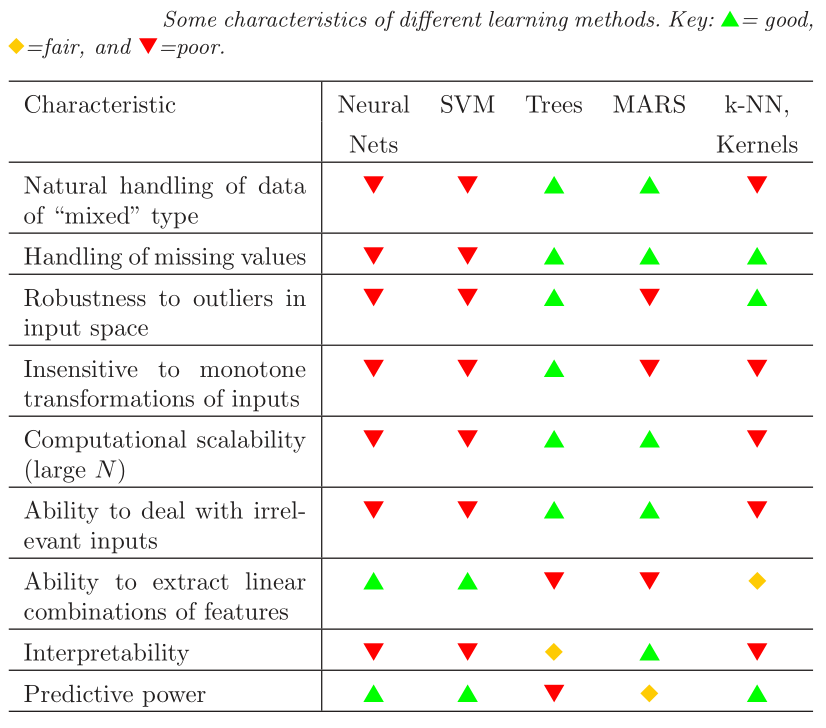
\includegraphics[scale=0.7]{method_comparison}
        \centering
        \caption {Comparison of Classifiers}
        \label{fig:classifier_comparison} %\ref{fig:classifier_comparison}
    \end{figure}
\end{document}